\documentclass[11pt]{article}
\usepackage[margin=.8in]{geometry}
\usepackage{amsmath,amssymb,graphicx,hyperref}
\setlength{\parindent}{0pt}\setlength{\parskip}{6pt}
\begin{document}
\begin{center}{\Large Actual asymmetric point contributions survive normalization}\\
23 November 2026 --- local unsigned Lean component evidence\end{center}
\textbf{Actual result.}
Retain the actual coefficient embedding, its cubic remainder \(A(X)+B(X)Y\),
actual short Weierstrass curve, nonsingular point \((x,y)\), nonzero two and
ordinate. Suppose the actual original mixed jets have opposite-branch orders
\(r_+,r_-\), and the original coordinate function is nonzero. Put
\(m=\min(r_+,r_-)\). Construct
\[
 A_{\rm new}=A/_{\rm monic}(X-x)^m,\quad
 B_{\rm new}=B/_{\rm monic}(X-x)^m,\quad h_{\rm new}=A_{\rm new}+B_{\rm new}Y.
\]
Lean derives an actual integral ideal \(J\) and exact equality
\[
 h_{\rm new}\ne0,\qquad
 \langle h_{\rm new}\rangle=I_+^{r_+-m}I_-^{r_--m}J.
\]
The ideal \(J\) and successful factorization are constructed, not supplied.
Nonzero original coordinate class remains an explicit premise
(PCC-20261123-1d0e6d) [pcc:unverified].
\begin{center}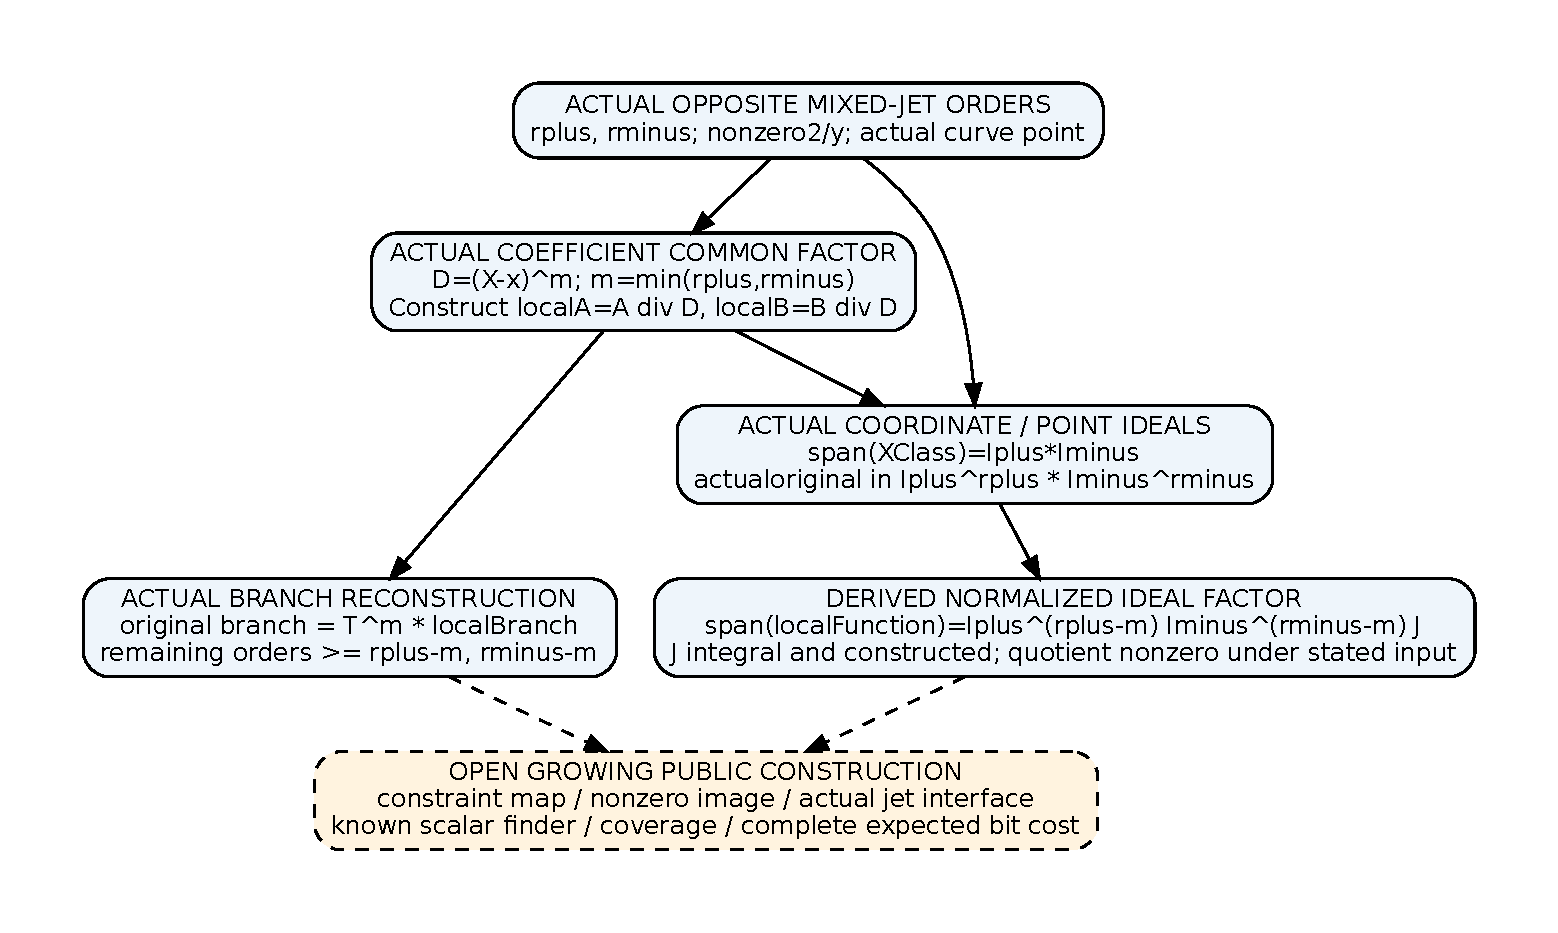
\includegraphics[height=4.5in,width=.98\linewidth,keepaspectratio]{asymmetric-normalization-dependencies-001.pdf}\end{center}
The powers are guaranteed contributions, not exact valuations or a greatest
common divisor assertion. The dashed boundary marks the growing public
construction and useful-scalar obligations still to establish.
\newpage
\begin{center}{\Large Actual maps and cancellation proof}\end{center}
\textbf{1. Unequal branch orders.}
The actual square-root branch is constructed from the stated point and unit
premises. Actual original substitutions on the two branches give norm order
at least \(r_++r_-\). Monotonicity of the actual mixed-jet predicate lowers
both orders to \(m\), and the accepted paired-coefficient theorem derives
\((X-x)^m\mid A,B\) [pcc:unverified].

\textbf{2. Constructed quotient and series factor.}
Public monic polynomial division reconstructs the actual coefficients from
\(A_{\rm new},B_{\rm new}\). Actual curve-remainder evaluation gives
\[
 h_{\rm original}(T,\pm s(T))=T^m h_{\rm new}(T,\pm s(T)).
\]
Nonzero \(T^m\) cancellation derives the normalized branch orders at least
\(r_+-m,r_--m\). No successful quotient or formal root is an input witness
[pcc:unverified].

\textbf{3. Actual point ideals.}
An explicit actual scalar and difference of the two \(Y\)-classes derive
coprimeness of \(I_+,I_-\). The existing actual mixed-jet-to-ideal theorem puts
the original coordinate function in \(I_+^{r_+}I_-^{r_-}\).
The public opposite-point ideal law gives
\(\langle X-x\rangle=I_+I_-\) [pcc:unverified].

\textbf{4. Integral residual and normalized ideal.}
The actual nonsingular points supply their actual invertible fractional ideal
units. The separately committed generic integral-residual theorem constructs
\(J\) with
\(\langle h_{\rm original}\rangle=I_+^{r_+}I_-^{r_-}J\).
Actual coordinate reconstruction gives
\(h_{\rm original}=(X-x)^m h_{\rm new}\).
Public singleton-ideal product/power laws and actual fractional unit
cancellation then derive the stated normalized ideal equality. Nonzero original
function implies nonzero quotient [pcc:unverified].

\textbf{Check map.}
The final run is source 088, build 094, local receipt 046:217 local statements,
twelve new since205, exit zero, zero warnings, all printed foundations standard.
All292 final input bindings are checked. The stages are:
\begin{center}\begin{tabular}{lll}
\textbf{Source/build}&\textbf{Local receipt}&\textbf{New scope}\\
082/088&043&actual norm sum and common minimum\\
084/090&044&constructed quotient and branch orders\\
085/091&045&actual coordinate and coprime ideals\\
088/094&046&actual normalized point-ideal factor
\end{tabular}\end{center}
PCC-20261123-26f39b,08ea66,c87435 and1d0e6d bind these stages and remain
unsigned local data outside the historical shared Transport53/57 audit/fresh
[pcc:unverified].
\newpage
\begin{center}{\Large Scope, controls, sources and next public construction}\end{center}
\textbf{Controls and limits of the conclusion.}
Equal orders \(r_+=r_-\) make both explicit surviving exponents zero. If one
order is zero, the other prescribed point power remains in the formula.
These are specializations of the derived general equality, not new empirical
runs. Extra vanishing may remain in \(J\); weakening equal-order constraints
does not establish exact asymmetric multiplicity. No primitive quotient or
maximal common-factor claim is made.

The result concerns the actual accepted coefficient embedding and its actual
coordinate function. It does not construct a nonzero witness for a new growing
asymmetric constraint family. In particular, the nonzero original coordinate
class premise has not been discharged for such a family. The integral \(J\)
is algebraically constructed; its efficient representation, rational splitting
and useful scalar labels are not conclusions [pcc:unverified].

\textbf{Next discriminating proof.}
Construct a growing public constraint map with an explicit finite coefficient
basis, actual degree budget and proved nonzero coordinate image. State whether
its constraints are original bivariate mixed jets or one-dimensional branch
jets. The current ideal-factor theorem uses the former; branch-only constraints
need their own actual point-ideal-power interface before substitution.

One source-backed interface to investigate is the actual truncated jet algebra
at a nonsingular rational point, with derived kernel \(I^n\), surjectivity and
dimension \(n\). The accepted actual point-power quotient dimension can supply
the dimension comparison. Public power-series truncation and nilpotent
polynomial quotient APIs are candidates, not a completed map. A formal
existence proof must not hide an efficient square-root or kernel-finder oracle.

After the actual map, retain all degree/coefficient/field/bit/entry and support
choice costs, bind the surviving known-point sum to useful scalar recovery,
and prove public finder coverage and retries. The earlier short residual
certificate coverage bounds and invariant residual class remain applicable at
their recorded scopes. None is a universal algorithm lower bound.

\textbf{Sources checked.}
The actual prior branch, coefficient remainder, mixed-jet/ideal and coordinate
class declarations are in the pinned parent source. Public Mathlib monic
division, cancellative divisibility, coprime ideal products, opposite-point
ideal/unit and singleton product/power laws are reused. Generic residual
construction is the committed owner module
\texttt{CryptoLean.InvertibleIdealResidual}.
Lean4.35.0 and Mathlib revision \texttt{cfc55fc} are pinned. KB access and
conductor remained unavailable as explicitly recorded; primary-source fallback
was used. No novelty claim is made for this standard algebra.

\textbf{Failure and artifact preservation.}
Rejected081 parser,083 reconstruction simplification and087 ideal permutation /
unit-API failures remain exact;086 is retained unlaunched after preflight
review. Final088 uses public explicit identities and removes only unused new
simp arguments. No private-body, linter, class, trust or resource override was
introduced. Prior source, evidence, raw, report and claim bytes and the local
ledger prefix remain exact; the protected canonical ledger conflict affects
remote publication only.
\end{document}
